%%% Example of a presentation using LaTeX-beamer theme for GI
%%% (c) Pierre Lemaire, 2015, 2016.
%%% Released under license CC-BY-SA 4.0 (https://creativecommons.org/licenses/by-sa/4.0/)
%%% Logos and images may be copyrighted. 

\documentclass[aspectratio=169]{beamer}
\setbeameroption{hide notes}

\usepackage[T1]{fontenc}
\usepackage[utf8]{inputenc}
\usepackage{pgfpages}
\usepackage{amsbsy} % bold math symbols

\usetheme[simple,itemshape=square,progressbar=yes]{GI}

\def\option#1{\texttt{\usebeamercolor[fg]{example text}#1}}%
\def\quote#1:#2<#3>{#3\par\bigskip\textit{\alert{\textbf{#1}}}
  \textit{\usebeamercolor[fg]{example text} #2}}


% === document info ===========================================================
\title[Format \LaTeX\ GI]{Format \LaTeX-beamer pour GI}%
\subtitle{(exemple d'utilisation)}
\author[]{Pierre Lemaire}%
\institute{Grenoble INP - Génie Industriel}
\date{juin 2016}%
\subject{présentation \LaTeX}
\keywords{format,beamer,\LaTeX}


\begin{document}

%% =============================================================================
\section[Introduction]{Introduction au thème GI}
\subsection{Un thème \LaTeX-beamer pour GI}

%% -----------------------------------------------------------------------------
\begin{frame}
  \frametitle{A propos de ce document}
  
  Ce document est une présentation \LaTeX\ réalisée avec la classe beamer et un thème adapté à GI

  \bigskip
  
  Ce document permet~:
  \begin{itemize}
  \item d'expliciter les options du thème
  \item de montrer un exemple de présentation ainsi obtenue (d'autres
    mises en forme sont données en annexe, à la fin du présent
    document)
  \end{itemize}
\end{frame}

%% -----------------------------------------------------------------------------
\frame{%
  \frametitle{Utilisation du thème}

  Le thème \LaTeX-beamer pour GI est disponible sur \url{http://www.kamick.org/lemaire/dev.html}

  \bigskip

  Les fichiers de définition du
  thème\footnote{\texttt{beamerthemeGI.sty},
    \texttt{beamercolorthemeGI.sty}} et les
  images\footnote{\texttt{bckgrd0.pdf}, \texttt{bckgrd1.pdf},
    \texttt{bckgrd2.pdf}} doivent être trouvés lors de la compilation

  \bigskip

  Il s'agit d'un thème \LaTeX-beamer, à utiliser comme tel

  Les sources de ce document donne des exemples d'usages

  \bigskip

  Pour plus d'informations sur \LaTeX-beamer~:

  \begin{thebibliography}{99}
  %\bibitem{} Donald E. Knuth, \textit{The \TeX book}, AMS, 1986.
  \bibitem{} Till Tantau et al., \textit{The \textsc{beamer} class user guide}, 2011.
  \end{thebibliography}
}

%% =============================================================================
\section[Options]{Options du thème}
% -----------------------------------------------------------------------------
\subsection{Mises en forme}
% -----------------------------------------------------------------------------
\frame{%
  \frametitle{Paramètres généraux}
  \begin{itemize}
  \item \option{none}~:   toutes les options à \option{none}
  \item \option{plain}~:  toutes les options à \option{plain}
  \item \option{simple}~: toutes les options à \option{simple}
  \item \option{fancy}~:  toutes les options à \option{fancy}
    \bigskip

    \begin{exampleblock}{\footnotesize Exemple}\footnotesize
      \string\usetheme[simple]\string{GI\string}
    \end{exampleblock}
  \end{itemize}
}

% -----------------------------------------------------------------------------
\frame[allowframebreaks]{%
  \frametitle{En-têtes et pieds de page}
  \begin{itemize}
  \item \option{headline}~: format de l'en-tête
    \begin{itemize}
    \item \option{none}~: n'ajoute pas d'en-tête
    \item \option{plain}~: ajoute un en-tête avec titres de sections
    \item \option{simple} (défaut)~: ajoute un en-tête avec auteur (court), titre (court), section courante, sous-sections
    \item \option{fancy}~: ajoute un en-tête avec titres de sections et ronds pour les diapositives
    \end{itemize}
    \smallskip
  \item \option{footline}~: format du pied-de-page
    \begin{itemize}
    \item \option{none}~: n'ajoute pas de pied-de-page
    \item \option{plain}~: ajoute un pied-de-page réduit avec uniquement les numéros de page
    \item \option{simple} (défaut)~: identique à \option{plain}
    \item \option{fancy}~: ajoute un pied-de-page avec auteurs (courts), titre (court) et numéros de page
    \end{itemize}
    \smallskip
    \goodbreak
  \item \option{framecount}~: format du numéro de diapo
    \begin{itemize}
    \item \option{none}~: aucun numéro de page (déconseillé)
    \item \option{plain}~: numéro de page seul
    \item \option{simple} (défaut)~: numéro de page et nombre total de pages
    \item \option{fancy}~: idem \option{simple}
    \end{itemize}
    \smallskip
  \item \option{progressbar}~: barre de progression
    \begin{itemize}
      \item \option{no} (defaut)~: n'ajoute pas de barre de progression sur le pied-de-page
      \item \option{yes}~: ajoute une barre de progression sur le pied-de-page
    \end{itemize}
  \end{itemize}
  \smallskip
  \begin{exampleblock}{\footnotesize Exemples}\footnotesize
    \string\usetheme[headline=none,progressbar=yes]\string{GI\string}

    \string\usetheme[fancy,framecount=plain,progressbar=yes]\string{GI\string}
  \end{exampleblock}
}

% -----------------------------------------------------------------------------
\frame{%
  \frametitle{Formes et couleurs}
  \begin{itemize}
  \item \option{colormode}~: couleurs du texte et des titres
    \begin{itemize}
    \item \option{plain}~: couleur de base noire
    \item \option{simple}~: couleur de base noire, bleue pour les titres
    \item \option{fancy}~: couleur de base bleue
    \end{itemize}

    \bigskip
  \item \option{itemshape}~: forme des puces (\option{ball}, \option{square}, \option{circle}, \option{default})
  \end{itemize}
  \bigskip
  \begin{exampleblock}{\footnotesize Exemples}\footnotesize
    \string\usetheme[colormode=plain,itemshape=ball
  \end{exampleblock}

}

% -----------------------------------------------------------------------------
\subsection{Comportements}
% -----------------------------------------------------------------------------
\frame{%
  \frametitle{Insertion automatique de diapositives}
  \begin{itemize}
  \item \option{titlepage}~: page de titre
    \begin{itemize}
    \item \option{auto} (défaut)~: ajoutée automatiquement (numérotée 0)
    \item \option{none}~: pas de page de titre (insertion manuelle par \texttt{\string\frame[t,plain]\string{\string\titlepage\string}})%

    \end{itemize}
    \bigskip
  \item \option{toc}~: tables des matières
    \begin{itemize}
    \item \option{none}~: aucune TOC ajoutée automatiquement
    \item \option{plain}~: TOC minimaliste pour chaque section
    \item \option{simple}~: TOC normale pour chaque section
    \item \option{fancy}~: TOC fantaisie ajoutée pour chaque sous-section
    \end{itemize}
  \end{itemize}
}

\frame{%
  \frametitle{Arrêt de numérotation}
  \begin{itemize}
  \item la macro \option{\string\lastframe} permet d'indiquer qu'une
    frame (la dernière insérée) doit être considérée comme la dernière
    et que les suivantes sont sur-numéraires. Très pratique pour
    exclure d'éventuelles annexes (usage~:
    \texttt{\string\lastframe\string\appendix}).
  \end{itemize}
}

%% =============================================================================
\section[Exemples]{Exemples de diapositives}

% -----------------------------------------------------------------------------
\subsection{Formatages de base}
% -----------------------------------------------------------------------------
\frame{%
  \frametitle{Texte et mises en formes} 

  \quote \hfill Vladimir Nabokov,:Lolita<Lolita, light of my life, fire
  of my loins. My sin, my soul.  \textbf{Lo-lee-ta: the tip of the
    tongue taking a trip of three steps down the palate to tap, at
    three, on the teeth.}  Lo. Lee. Ta.>

  % She was Lo, plain Lo, in the morning, standing four feet ten in one
  % sock. She was Lola in slacks. She was Dolly at school.  She was
  % Dolores on the dotted line. But in my arms she was always Lolita.

  % Did she have a precursor? She did, indeed she did. In point of fact,
  % there might have been no Lolita at all had I not loved, one summer,
  % a certain initial girl-child. In a princedom by the sea. Oh when?
  % About as many years before Lolita was born as my age was that
  % summer. You can always count on a murderer for a fancy prose style.

  % Ladies and gentlemen of the jury, exhibit number one is what the
  % seraphs, the misinformed, simple, noble-winged seraphs, envied.
  % Look at this tangle of thorns.
}

% -----------------------------------------------------------------------------
\frame{%
  \frametitle{Listes} 
  \begin{itemize}
  \item Jane Austen
    \begin{itemize}
    \item Pride and Prejudice
    \item Mansfield Park
    \end{itemize}
  \item Jorge Luis Borges
    \begin{itemize}
    \item Ficciones
    \item El libro de arena
    \end{itemize}
  \item Bertolt Brecht
    \begin{itemize}
    \item Dans la jungle des villes
    \item La Résistible ascension d'Arturo Ui
    \item Mère Courage et ses enfants
    \item L'Opéra de quat'sous
    \item La Vie de Galilée
    \end{itemize}
  \end{itemize}
}
% -----------------------------------------------------------------------------
\frame{%
  \frametitle{Énumérations} 
  \begin{enumerate}
  \item Fédor Dostoïevski
    \begin{enumerate}
    \item L'Idiot
    \item Le Double
    \item Le Joueur
    \item Les Frères Karamazov
    \end{enumerate}
  \item Jasper Fforde
    \begin{enumerate}
    \item The Eyre Affair
    \item The Big Over Easy
    \item Shades of Grey
    \end{enumerate}
  \item Friedrich Nietzsche
    \begin{enumerate}
    \item Ainsi parlait Zarathoustra
    \item Le Gai Savoir
    \end{enumerate}
  \end{enumerate}
}

% -----------------------------------------------------------------------------
\frame{%
  \frametitle{Colonnes}
  \begin{columns}
    \begin{column}{.55\textwidth}\raggedright
      \quote François Villon\\:Quatrain<Je suis François, dont ce me poise,\\%
      Né de Paris emprès Ponthoise. \\%
      Or d‘une corde d’une toise \\%
      Saura mon col que mon cul poise.> %
    \end{column}
    \begin{column}{.45\textwidth}\raggedleft
      \quote Bertolt Brecht\\:L'Opéra de quat'sous<Au bout d'une corde
      de plusieurs aunes son cou ressent ce que pèse son cul.\\~>
    \end{column}
  \end{columns}
}

% -----------------------------------------------------------------------------
\subsection{Cadres}
\frame[allowframebreaks]{%
  \frametitle{Blocs de texte}

  \begin{alertblock}{Vladimir Nabokov}
    \quote :<Mes aversions sont simples : la stupidité, l'oppression,
    le crime, la cruauté et la musique douce.\\\kern-2.25ex>
  \end{alertblock}

  \begin{block}{Jacques Prévert}
    \quote:<Il faudrait essayer d'être heureux, ne serait-ce que pour
    donner l'exemple.\\\kern-5ex>
  \end{block}

  \begin{exampleblock}{Jens Peter Jacobsen}
    \quote:<Eux-mêmes parlaient avec
    une rigidité de syntaxe qui faisait en quelque sorte saillir à
    travers leurs phrases les côtes de la grammaire.>

    \quote:<Grandissantes, les ombres dans la pièce sortaient une à
    une des meubles et des murailles.\\\kern-5ex>
  \end{exampleblock}

  \begin{block}{}\centering
    \quote Ryszard Kapu\'sci\'nski,:Le Négus<Il ne manifesta jamais
    aucun penchant pour la corruption, attitude qui lui valut des
    années d'emprisonnement et, pour finir, la décapitation.\\\kern-2.25ex>
  \end{block}
}

% -----------------------------------------------------------------------------
\subsection[Divers]{Formatages divers}
% -----------------------------------------------------------------------------
\def\x#1#2{#2 \alert{(#1)}}
\frame{%
  \small
  \frametitle{Exemple complet}
  \begin{alertblock}{}\centering%
    \x{Nietzsche}{Que serait ton bonheur, si tu n'avais ceux que tu
      éclaires~?}
  \end{alertblock}
  \begin{columns}
    \begin{column}{.5\textwidth}
      \begin{enumerate}
      \item \x{Ferré}{Le Bonheur, ça n'est pas grand chose ... c'est
          du chagrin qui se repose.}
      \item \x{Lenoir}{Le «droit» au bonheur s'est mué en «devoir» et,
          du coup, en fardeau.}
      \end{enumerate}
    \end{column}
    \begin{column}{.5\textwidth}
      \begin{exampleblock}{}\footnotesize
        \x{Schopenhauer}{Ce que quelqu'un possède pour soi, ce qui
          l'accompagne dans la solitude et que personne ne peut lui
          donner ni lui prendre, voilà qui est beaucoup plus essentiel
          que tout ce qu'il possède ou ce qu'il est aux yeux des
          autres.}
      \end{exampleblock}
    \end{column}
  \end{columns}  
  \begin{columns}
    \begin{column}{.6\textwidth}
      \x{Flaubert}{Être bête, égoïste et avoir une bonne santé : voilà
        les trois conditions voulues pour être heureux. Mais si la
        première nous manque, tout est perdu.}
    \end{column}
    \begin{column}{.4\textwidth}\footnotesize
      \begin{itemize}
      \item \x{Cohen}{Au bout du compte, la page reste toujours
          blanche du bonheur à conquérir.}
      \item \x{Huxley}{Happiness is never grand.}
      \end{itemize}
    \end{column}
  \end{columns}  
}

% -----------------------------------------------------------------------------
\frame[t]{%
  \frametitle{Diapo avec texte en haut}
  \quote Albert Camus\\:La Chute<Un balcon naturel, à cinq ou six cents
  mètres au dessus de la mer encore visible et baignée de lumière,
  était au contraire l'endroit où je respirais le mieux, surtout si
  j'étais seul, bien au-dessus des fourmis humaines.>
}

% -----------------------------------------------------------------------------
\frame[b]{%
  \frametitle{Diapo avec texte en bas}

  \raggedleft
  \quote Friedrich Nietzsche\\:Ainsi parlait Zarathoustra<J'ai devant
  moi ma cime la plus haute et mon pèlerinage est le plus long ; c'est
  pourquoi il me faut d'abord descendre plus bas que je ne descendis
  jamais.> 
}


% -----------------------------------------------------------------------------
\frame{%
  \frametitle{Format des diapos}

  Le thème est compatible avec l'option \option{aspectratio} de beamer~:

  \noindent
  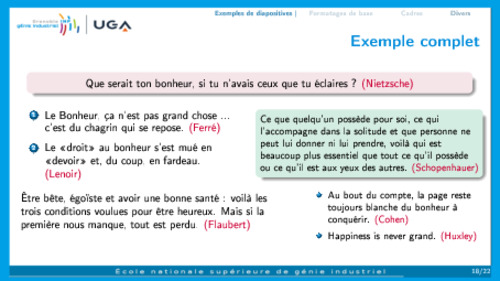
\includegraphics[width=.32\textwidth]{Img/zz24}%169
  \hfill
  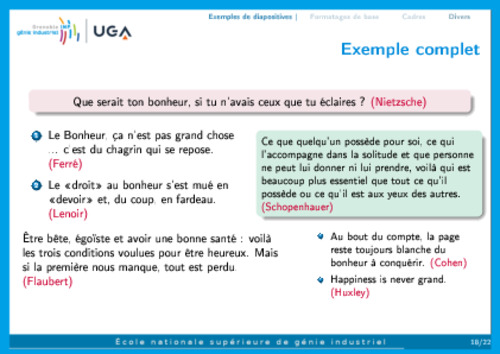
\includegraphics[width=.32\textwidth]{Img/zz26}%141
  \hfill
  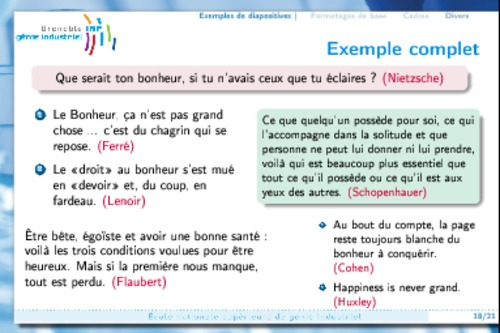
\includegraphics[width=.32\textwidth]{Img/zz29}%32

  aspectratio=169
  \hfill
  aspectratio=141
  \hfill
  aspectratio=32
  \goodbreak
}

\frame{
  \centering
  \quote Alexandre Soljenitsyne:Le pavillon des cancéreux<Le sot aime à faire la leçon, le malin préfère la recevoir.>
}

\lastframe
\appendix
\section{Annexes}
\subsection[Options]{Exemples de choix d'options}

\def\x#1#2{%
  \centering
  \begin{exampleblock}{}\scriptsize
    \string\usetheme[\alert{#2}]\string{GI\string}%
  \end{exampleblock}
  \includegraphics[height=.7\textheight]{Img/zz#1}%
  \goodbreak
  
}
\frame[b,allowframebreaks]{
  \x{1}{none}
  \x{2}{plain}
  \x{3}{simple}
  \x{4}{fancy}
  \x{5}{plain,colorstyle=fancy}
  \x{6}{fancy,colorstyle=simple,progressbar=yes,framecount=plain}
  \x{7}{simple,headline=none,footline=plain,itemshape=square}
  \x{8}{none,progressbar=yes,colorstyle=fancy}
}


% \subsection[Tailles]{Exemples de choix de tailles de diapos}
% \def\x#1#2#3{%
%   \centering
%   \begin{exampleblock}{}\scriptsize
%     \string\documentclass[aspectratio=\alert{#3}]\string{beamer\string}%
%     \string\usetheme[\alert{#2}]\string{GSCOP\string}%
%   \end{exampleblock}
%   \includegraphics[height=.7\textheight]{Img/zz#1}%
%   \goodbreak
  
% }
% \frame[b,allowframebreaks]{
%   \x{9}{none,progressbar=yes}{1610}
%   \x{10}{none,progressbar=yes}{169}
%   \x{11}{none,progressbar=yes}{149}
%   \x{12}{none,progressbar=yes}{141}
%   \x{13}{none,progressbar=yes}{54}
%   \x{14}{none,progressbar=yes}{43}
%   \x{15}{none,progressbar=yes}{32}

%   \x{16}{plain,progressbar=yes}{1610}
%   \x{17}{plain,progressbar=yes}{169}
%   \x{18}{plain,progressbar=yes}{149}
%   \x{19}{plain,progressbar=yes}{141}
%   \x{20}{plain,progressbar=yes}{54}
%   \x{21}{plain,progressbar=yes}{43}
%   \x{22}{plain,progressbar=yes}{32}


%   \x{23}{simple,progressbar=yes}{1610}
%   \x{24}{simple,progressbar=yes}{169}
%   \x{25}{simple,progressbar=yes}{149}
%   \x{26}{simple,progressbar=yes}{141}
%   \x{27}{simple,progressbar=yes}{54}
%   \x{28}{simple,progressbar=yes}{43}
%   \x{29}{simple,progressbar=yes}{32}

%   \x{30}{fancy,progressbar=yes}{1610}
%   \x{31}{fancy,progressbar=yes}{169}
%   \x{32}{fancy,progressbar=yes}{149}
%   \x{33}{fancy,progressbar=yes}{141}
%   \x{34}{fancy,progressbar=yes}{54}
%   \x{35}{fancy,progressbar=yes}{43}
%   \x{36}{fancy,progressbar=yes}{32}
% }



\end{document}

